\chapter{Tracking system components}
The main goal of our project is to design and implement a system that can determine the exact position of each moving object at any time. The mentioned system should be cost-effective in addition to proper performance.\\
To design such a system, we must first identify the system requirements and the overall architecture of the system we want. Then we use this architecture to implement the appropriate modules. In this chapter, in section 2.1, we first explain the general design of the tracking system and then in section 2.2, we introduce the components used in this design.

\section{System design and architecture}
In this section, we will design our system. According to the project's requirements, we must specify the transmitter and receiver modules, communication protocol, and application program for displaying information. The primary purpose of a tracking system is to track a specific object and gain its path. The tracking system provides information about the current location and speed of the object.\\
In this project, our communication has been one-way, in which the coordinates of the moving object are continuously measured and sent to a server. Then, the necessary processing of this information is performed on the server-side. According to the above explanations, we can mention three main parts in this system \cite{5}:
\begin{itemize}
	\item Obtain the location of a moving object using the GPS module
	\item Send location information to software servers by GSM modem
	\item Store location information on the server-side and implement an application to display the object's path on the map
\end{itemize}
As we have seen, the architecture of our system has four main parts. The first part is about locating the object from the satellite using the GPS module. The second part is related to sending the received information to the server using a GSM modem. The third part is the development of an application that uses the received data to display the location of the object on the map.\\
\begin{figure}[!h]
	\centerline{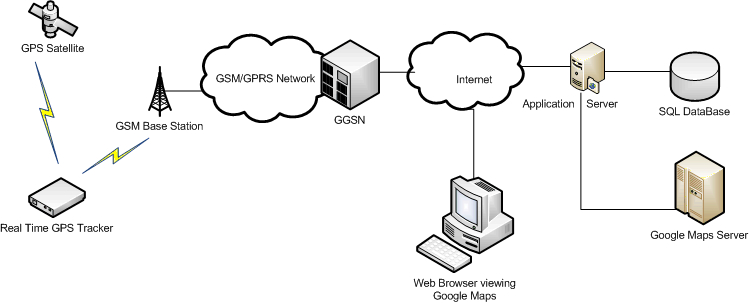
\includegraphics[width=.8\textwidth]{GPS_Tracker}}
	\caption{Block Diagram of Tracking System \cite{6}}
\end{figure}\\
Figure 2.1 shows an overview of the designed system architecture and the relationship between its parts. ّFor selecting the modules, it is necessary to know the task of each section accurately and choose the desired module for it \cite{7}.
\begin{itemize}
	\item In the first part, we need to measure the location of the object continuously. As soon as the object moves, the GPS module consistently receives the moving object's coordinate from the satellite. The signal received from the satellite is weak, so we must use an antenna to amplify the desired signal, and at the end, sends the amplified signal to the Arduino board.
	\item In the second part, the information received from the GPS module is sent to the server by the GSM modem.
	\item Software servers analyze the information after receiving them. Our communication in this project is one-way, and we will not have a request from software servers. In this part of the project, web-based software will be developed to process the submitted information and store them in the database. In the last section, this information will be displayed in the designed web page.
\end{itemize}
\begin{figure}[!h]
	\centerline{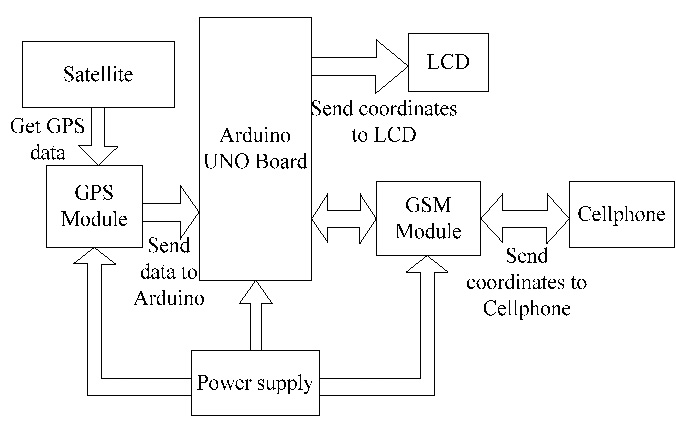
\includegraphics[width=.6\textwidth]{blockdiagram}}
	\caption{Architecture of Tracking System\cite{3}}
\end{figure}
\section{System components}
In the previous section, we defined the system architecture. Now we will express and introduce the components of this architecture in detail.
\subsection{Hardware components}
The hardware components used to implement this system are:
\begin{itemize}
	\item Arduino module
	\item SIM808 module
	\item GPS antenna
	\item GSM modem
\end{itemize}
\subsubsection{Arduino module}
Arduino is an open-source microprocessor suitable for writing applications that interact with the environment and objects outside. This board is ideal for prototyping, and its software and hardware design are freely available to all people. Any interested person, even with a little knowledge and experience in electronics, can use Arduino to do their projects.\\
Arduino has a simple programming environment that anyone with a little knowledge of C and C++ can program in this environment and run the program written in Arduino. Various sensors can be connected to the Arduino microcontroller and controlled. The microprocessor used on the Arduino board is based on the Arduino programming language and does not require any additional software or compiler for coding.\\
Figure 2.3 shows the Arduino Uno board:
\begin{figure}[!h]
	\centerline{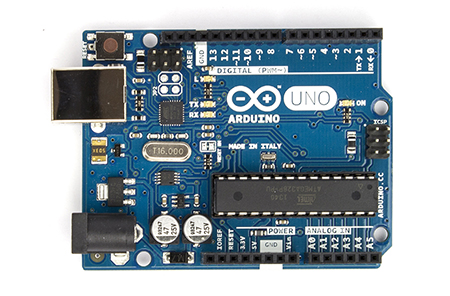
\includegraphics[width=.5\textwidth]{ArduinoUno_R3}}
	\caption{Arduino Uno board}
\end{figure}
\subsubsection{SIM808 module}
The 808 SIM module is a combination of GSM / GPS PRS 9 module and GPS module with 1900 MHz support for data transmission, SMS and voice calling.
This module has a SIM card socket in which the SIM card is inserted. Using the GSM / GPRS modem and the 808 SIM module, you can exchange data over the GSM network via the USB interface and access the information of devices located in remote locations.\\
In figure 2.4, You can see this chip.
\begin{figure}[!h]
	\centerline{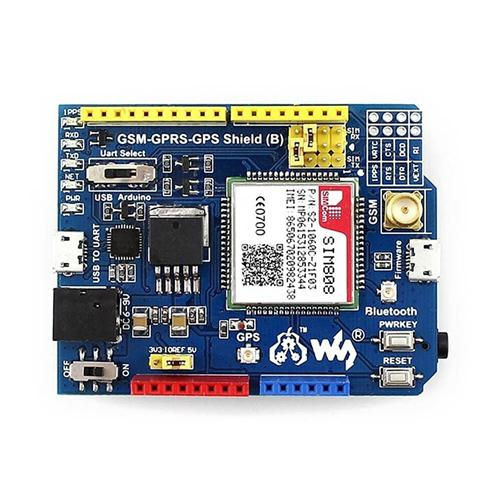
\includegraphics[width=.5\textwidth]{sim809}}
	\caption{SIM 808 module}
\end{figure}
\subsection{Software components}
\subsubsection{Arduino IDE}
The software used for programming is Arduino software, which you can see in Figure 2.5. Using the C language, you can write the required program, and after compiling, the generated hex code is uploaded on the Arduino. There are different libraries that make coding easier. The program is written using this software to receive data from satellite and send it to a mobile phone.\\
\begin{figure}[!h]
	\centerline{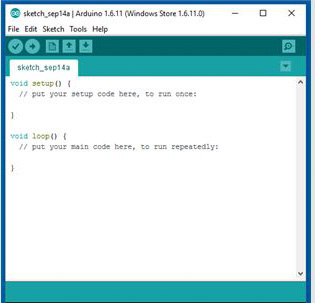
\includegraphics[width=.5\textwidth]{arduino-ide}}
	\caption{Arduino IDE}
\end{figure}